\documentclass{ltjsbook}
\usepackage{docmute} 
\usepackage{../../myStyle} 

\begin{document}
\setcounter{chapter}{9}
\chapter{システム論からみた社会心理学：第四世代システム}
\label{sp10_system}

\section{導入}

それでは，今日のお話をしたいと思います。これは第10回目です。現在は第2部ということで，システム論の話をしています。今日は第5世代システムのところまで言及して終わらせたいと思っています。ただ，時間的には厳しいかもしれないので，次週にちょっとずれ込むところもあるかもしれません。そんな感じで進めていきたいと思います。

前回までの講義録も，先日LMSの方にアップロードしました。教室に来られている方よりも，レポートの数が圧倒的に多いので，おそらく受講生はそれを読んでいただいていると思います。前回のシステム論の話，授業中に喋っている内容があやふやな記憶だとか，その場の勢いで喋っているところがあって。お恥ずかしいやら，申し訳ないやら。見直して間違ったことを言っているなと思う部分は，文字起こしするときに補正をかけています。出典，引用等も付いていますので，この話がよくわからないと思うところがあったら，そのあたりを読み直していただければと思います。

私も喋りながらなので，熱があるような話し方をすると話し言葉ですので，同じことを繰り返したり，同じ発言が多くなってしまうことがあります。文字起こしを校正するのもそこそこ大変なんですが，ともかく，校正の段階で話す部分がカットされてしまうこともあります。ですから，それぞれの章の分量も様々です。まあ講義録も参考にしていただければと思います。

逆に，ライブで聞いていただいている皆さんにとっての価値は何かというと，表情が見えて熱がどこに入ってるか，重点を置いてる場所のヒントとか，ジェスチャーが見れるとか，図の参照がリアルタイムにできるという点ですかね。まあ皆さんに損をさせないように，面白い話題を提供できればと思っています。頑張ります。

\subsection{動的非平衡系のまとめ}

前回は第二世代システム\index[termidx]{だいにせだいしすてむ@第二世代システム}，第三世代システム\index[termidx]{だいさんせだいしすてむ@第三世代システム}の話をしました。第二世代システム\index[termidx]{だいにせだいしすてむ@第二世代システム}は動的非平衡あるいは自己組織化系\index[termidx]{じこそしきかけい@自己組織化系}ということで，システムがどのように自己を作っていくのかという話をしました。その時のいくつか新たな視点の導入がありました。1つは自己組織化系\index[termidx]{じこそしきかけい@自己組織化系}という別名がヒントですね。第一世代システム\index[termidx]{だいいちせだいしすてむ@第一世代システム}はインプットとアウトプットを繰り返しながら，安定するものとしてシステムを考えようと言ってましたね。この安定する点，システムの目的を誰がどう作っているのかというようなことを，システムの自己の組織化，自分で作っていくものとして話をしました。安定するポイントを自分で作っていくのです。その話の中に入っているのが，実は階層的な関係です。ミクロ的なレベルでは非平衡的なんだけど，マクロな視点で見ると安定しているというようなことです。また，時間の矢\index[termidx]{じかんのや@時間の矢}の話もしました。エントロピーは増大する方向にしか行かないので，化学反応や自己組織化\index[termidx]{じこそしきか@自己組織化}がスタートすると，不可逆的な，一方向的な変化をします。そういう時間の考え方も含まれているという自己組織化系\index[termidx]{じこそしきかけい@自己組織化系}という話をしました。

社会心理学的にも，そういったミクロなレベルとマクロなレベルというのは，最初から入っていますし，不可逆な相転移\index[termidx]{そうてんい@相転移}が生じるような現象というのもあるんじゃないか。こうやって考えるヒントになるんじゃないか，という話もしたかと思います。

\subsection{自己創出系のまとめ}

それが進みまして，第三世代システム\index[termidx]{だいさんせだいしすてむ@第三世代システム}として，第一世代オートポイエーシス\index[termidx]{おーとぽいえーしす@オートポイエーシス}という考え方が出てくるわけですね。

オートポイエーシス\index[termidx]{おーとぽいえーしす@オートポイエーシス}システムというのは，自己創出系という言われることがあります。システムというものが自分を自分で作っていくんですよという話は，第二世代の時にしていたんですが，それにしたところで，システムの観察者が外部に存在してたんですね。外部から見て，これが全体的なパターンであると言っていたんですが，オートポイエーシス\index[termidx]{おーとぽいえーしす@オートポイエーシス}を提唱したマトゥラーナとヴァレラ\index[nameidx]{ゔぁれら@ヴァレラ}はそうではなくて，システムを内側から見る。システムというのは，生命というのは，自律しているし，個体であるし，環境を自分で作っている。その境界を作り出そうというシステムが動いている以上は，入力も出力もないという言い方をしたことによって，新しいシステムの視点を提供したわけです。

ただし，入力も出力もないという言い方が，まるで第一世代システム\index[termidx]{だいいちせだいしすてむ@第一世代システム}の入力と出力という言葉，あるいは発想と真逆すぎたものですから，非常な混乱が生まれたんだという話をしました。

さて，オートポイエーシス\index[termidx]{おーとぽいえーしす@オートポイエーシス}に関する本はいくつかご紹介していましたが，今日ここに持ってきたのは，マトゥラーナと自身が書いた「オートポイエーシス\index[termidx]{おーとぽいえーしす@オートポイエーシス}」です\parencite{Maturana_Varela}。私は普段この授業では，河本英夫\index[nameidx]{かわもとひでお@河本英夫}の「オートポイエーシス\index[termidx]{おーとぽいえーしす@オートポイエーシス}」\parencite{KawamotoHideo}，の方を元に解説していました。システムを第一，第二，第三という時代で区分したのも彼です。「オートポイエーシス\index[termidx]{おーとぽいえーしす@オートポイエーシス}」\parencite{Maturana_Varela}を訳したのも河本英夫\index[nameidx]{かわもとひでお@河本英夫}ですね。こちらの本でマトゥラーナとヴァレラ\index[nameidx]{ゔぁれら@ヴァレラ}が，自身の言葉で，この考え方が提案されています。

それともう一つ，高校生向けと言われている「知恵の樹」という本も持ってきました\parencite{Chienoki}。これが今，文庫本になっていますし，一応読みやすいということになってるんです。どこから読んでも全体像がわかるからいいよということで，本の目次のページには，章ごとの関係を繋いだ図が載ってます。どういうフローチャートで読んでいったらよいかというのは，この図をみると多少繋がりがわかるんですが，とはいえどこから読んでも全体がわかるよということを意図して書かれているようです。興味があったら読んでみてください。

さて，これらの本に代表されるように，「生きているとは何であるか」ということを中心に，システムの考え方を提示してあるわけです。それでも，オートポイエーシス\index[termidx]{おーとぽいえーしす@オートポイエーシス}の限界があります。ここに藤澤等\index[nameidx]{ふじさわひとし@藤澤等}の「複合システムネットワーク\index[termidx]{ふくごうしすてむねっとわーく@複合システムネットワーク}論」という本があるのですが\parencite{fujisawaNetwork}，この本からオートポイエーシス\index[termidx]{おーとぽいえーしす@オートポイエーシス}というシステムの特徴を改めてまとめつつ，どこに問題があったのかを見ていきたいと思います。

\subsection{オートポイエーシスの限界}

藤澤が指摘するオートポイエーシス\index[termidx]{おーとぽいえーしす@オートポイエーシス}の特徴は次のようになります。

まず，システムは作動するプロセスであって，要素が作動によって生成されるようなものになっているシステムだということですね。ベルタランフィー\index[nameidx]{べるたらんふぃー@ベルタランフィー}の一般システム論ですとか，プリゴジン\index[nameidx]{ぷりごじん@プリゴジン}なんかが言ったような化学，熱統計的学なんかでのシステムというのは，(物理的)要素がどのように変化していくかという話をしているんです。しかし，オートポイエーシス\index[termidx]{おーとぽいえーしす@オートポイエーシス}に至って大きく変わったのは，システムはその産出の要素と要素をつないでいるプロセスの問題であって，このプロセスをするために，プロセスが続いていく過程によって，要素のほうが作られるんだという考え方をするという話です。この要素間の関係は，このプロセスがループをしたとき，循環的に状態が定まっていくという発想で，システムの境界はシステム自身が決めるんだということにつながります。

第一世代システム\index[termidx]{だいいちせだいしすてむ@第一世代システム}のように，外から見て「これがシステムですよ」というのではなくて，システム自身が自分のシステムとしてのひとまとまりの単位を作り出すのだということを言うわけです。また，オートポイエーシス\index[termidx]{おーとぽいえーしす@オートポイエーシス}というシステムの目的は一体何かというと，自分を再生産することにある。自己創出，自分を作るプロセスを維持するということが目的なんだという話をしていたわけです。

システム間の関係，システムとシステム，複数のシステム，生命と生命があったら，それがどういう関係になっているかということについては，オートポイエーシス\index[termidx]{おーとぽいえーしす@オートポイエーシス}の論者で意見が統一されてません。マトゥラーナとヴァレラ\index[nameidx]{ゔぁれら@ヴァレラ}のキーワードとしては「カップリング\index[termidx]{かっぷりんぐ@カップリング}している」という言い方をしています。このカップリング\index[termidx]{かっぷりんぐ@カップリング}あるいは，相互に浸透しているというような言い方がどういう意味なのかは，意見が分かれるところがあるようです。というのもオートポイエーシス\index[termidx]{おーとぽいえーしす@オートポイエーシス}は，基本的には単体としての孤立したシステムを中心に考えていますから，複数のシステムがどうなっているかということについては，明確に語られていないことが，良くも悪くもオートポイエーシス\index[termidx]{おーとぽいえーしす@オートポイエーシス}論の特徴だろうということです。

また，システムはシステムの外部からは観察されるものではない。観察者の視点がシステムの内側に移ったところがポイントになっています。オートポイエーシス\index[termidx]{おーとぽいえーしす@オートポイエーシス}のシステムがどういうことを問題提起したかと言いますと，要素というのを特定せずに，システムをどのように「これがシステムです」というふうに記述するのかという問題を論じたわけです。外部から見ていて，「これが要素です，これが全体です」というような規定をどう考えればよいのかという話をしている。あるいはシステムが自己というのをどのようにして決定するのか，要素関係の質は誰がどのように決定するのか，要素と全体の関係はどうなっているのかというようなところが，オートポイエーシス\index[termidx]{おーとぽいえーしす@オートポイエーシス}システムの中ではまだ問題として残っているといえるでしょう。

それを踏まえて，このシステム論の限界はですね，まず理論的な全体像が明確でないということです。マトゥラーナとヴァレラ\index[nameidx]{ゔぁれら@ヴァレラ}は，構造的カップリング\index[termidx]{こうぞうてきかっぷりんぐ@構造的カップリング}している複数のシステムがあったという時に，意見がちょっと分かれているんでしたね。河本も頑張って何か説明しようとしているようですが，ちょっとその説明も僕は分かりにくい印象があります。ルーマン\index[nameidx]{るーまん@ルーマン}も相互浸透ということで，社会のことを社会システム\index[termidx]{しゃかいしすてむ@社会システム}としてのオートポイエーシス\index[termidx]{おーとぽいえーしす@オートポイエーシス}を論じているわけですけれども，あくまでもそういう見立てですというところであって，彼も社会システム\index[termidx]{しゃかいしすてむ@社会システム}と個人システムがどのように関係しているのかということについては，まだ明確に語られていないということです。

あと，オートポイエーシス\index[termidx]{おーとぽいえーしす@オートポイエーシス}の最大の弱点は，数学的な記述がないということですね。ベルタランフィ\index[nameidx]{べるたらんふぃ@ベルタランフィ}は連立微分方程式\index[termidx]{れんりつびぶんほうていしき@連立微分方程式}というのにすることによって，一般システム論にしたわけです。一般化できる数学的な記述をすることによって，学際的な研究ができるんだということを売り切りしていたわけです。なぜ連立微分方程式\index[termidx]{れんりつびぶんほうていしき@連立微分方程式}だったかというと，当時はその数学だったら何とかアプローチできるだろうと，現代ほど離散数学は進んでなかったからということもあります。

ちなみに，第二世代システム\index[termidx]{だいにせだいしすてむ@第二世代システム}の自己組織化系\index[termidx]{じこそしきかけい@自己組織化系}とかっていうのは差分システムです。微分と差分の違いは，連続的に変わるのかどうかです。$t-1$時点の状態が$t$時点の状態に影響を及ぼす，前回の状態に変化して次の状態になる(ex.$x^{t+1}=x^t+e$)というのが離散的な動き方で，これが第二世代システム\index[termidx]{だいにせだいしすてむ@第二世代システム}の数学的な記述です。その記述は河本の本\parencite{KawamotoHideo}に書いてあります。

一方で，オートポイエーシス\index[termidx]{おーとぽいえーしす@オートポイエーシス}に至っては数学的な表現が一切ございません。マトゥラーナとヴァレラ\index[nameidx]{ゔぁれら@ヴァレラ}の本を読んでも，知恵の樹を読んでも，そのあたりは書いてません。社会心理学系の論文にオートポイエーシス\index[termidx]{おーとぽいえーしす@オートポイエーシス}を扱った論文\parencite{NomuraTatsuya}があったんですが，その著者とお会いしたときに，「オートポイエーシス\index[termidx]{おーとぽいえーしす@オートポイエーシス}はシステム論としていいんだけど，数式で書いてくれないから困るんだ」みたいなことをすごく語っておられたのを覚えてます。

数学的な記述がないということは，一般化しにくい，あるいは議論が十分に精緻化できていないという問題が含まれるわけですね。あとは，複数の問題の性質が混在していて，きれいに切り分けられていないんじゃないか，特に観察者がどこにいるのかという説明が十分に意識されていないのではないかというあたりが問題点として挙げられるかと思います。

社会心理学の文脈において，システム論あるいはオートポイエーシス\index[termidx]{おーとぽいえーしす@オートポイエーシス}を考えるときは，マトゥラーナとヴァレラ\index[nameidx]{ゔぁれら@ヴァレラ}が考えていた生命としての個体性，一単位で独立しているという状態だけを考えることは当然できないですね。システムが一個じゃないわけです。社会心理学をやるという意味では，個人が集まって社会になっているというところから始めざるを得ません。ルーマン\index[nameidx]{るーまん@ルーマン}のように社会学として，社会があって社会の学，社会のロジックだけだったらいいんですが，社会心理学を考えると，社会のレベルと個人のレベルの両方があって，それがどういった関係にあるのかということをやっぱり考えないわけにはいかない。

マトゥラーナとヴァレラ\index[nameidx]{ゔぁれら@ヴァレラ}は，それは適当にカップリング\index[termidx]{かっぷりんぐ@カップリング}してるんでしょう，みたいな表現の仕方をしているんですけど，やっぱり社会心理学をやる上では，そこがどういう関係なのかをしっかりと詰めていかないといけない。そもそも複数のシステムを前提しないといけない，というのが社会心理学の扱う問題の前提ですね。

私は「私」というシステムです。でも一人では社会ではないので，複数の人間がいたときに人が交わって公的なものができるから社会になるんだ，という話をいつしかしたと思います。複数のシステムがあるという前提から話をしないといけないので，オートポイエーシス\index[termidx]{おーとぽいえーしす@オートポイエーシス}の話をそういった方向で拡張していくというのが，今からやっていかないといけないところなわけです。

オートポイエーシス\index[termidx]{おーとぽいえーしす@オートポイエーシス}においても，複数のシステムがあることを，複合システム\index[termidx]{ふくごうしすてむ@複合システム}という言い方します。それについて，マトゥラーナは，システムは外部とカップリング\index[termidx]{かっぷりんぐ@カップリング}しているんだという話をしています。ヴァレラ\index[nameidx]{ゔぁれら@ヴァレラ}は細胞とか免疫とか神経システムといった，生物の問題の領域を定めてオートポイエーシス\index[termidx]{おーとぽいえーしす@オートポイエーシス}を論じ，複数のシステムについてはごく部分的にだけ扱えるものだと理解しているようです。ルーマン\index[nameidx]{るーまん@ルーマン}は複数のシステムが浸透し合っていて，個人のシステムと社会のシステムはその濃度が違うんだよという表現をしています。しかし，「その濃度って何？」ということについては，ちょっとよくわからない状態になっています。

河本\parencite{KawamotoHideo}の「構造的カップリング\index[termidx]{こうぞうてきかっぷりんぐ@構造的カップリング}」の説明の仕方は，複合システム\index[termidx]{ふくごうしすてむ@複合システム}のあり方は3パターンしか考えられないと述べています。複数のシステムがあった時，(1)一方が他方に従属している。上と上下の関係があると考えるか，(2)下のレベルの複数の個別のシステムがばらばらにあって，上位のシステムはオートポイエーシス\index[termidx]{おーとぽいえーしす@オートポイエーシス}ではないというような考え方をするか，(3)上位と下位は上位のシステムの様子が下位のシステムだというような考え方を取らないとするか。この3つだと述べています。このようなアプローチをしないと，複数の社会があるだとか，階層的にシステムが連なっているという話は，整合的に理解できないでしょうと言及するにとどまっています。

こういったシステム論では今まで考えてこられなかったであろう特徴が，社会心理学の中では複合的であること，階層的であることが，前提条件としてある中心問題になるわけですから，そういったシステム論について考えていかねばなりません。

\section{第四世代システム；複雑系}

このあたりのお話を今からやっていこうと思いますが，一足飛びに進むのではなく，今日はちょっと手前に第四世代システム\index[termidx]{だいよんせだいしすてむ@第四世代システム}として複雑系\index[termidx]{ふくざつけい@複雑系}の話をしたいと思います。複雑系\index[termidx]{ふくざつけい@複雑系}です。

今日お持ちしたのは，ミチェル・ワールドロップ\index[nameidx]{わーるどろっぷ@ワールドロップ}という人が書いている「複雑系\index[termidx]{ふくざつけい@複雑系}」という本です\parencite{Waldrop}。これもたぶん今確か文庫になっているので，興味がある人は読んでみてください。「知恵の樹」\parencite{Chienoki}の何倍も読みやすいです。というか，これはどちらかというと，サイエンス読み物ですね。論文だとか専門書というのとは違い，科学的な読み物として書かれています。すごくお話として読みやすいです。

皆さん，複雑系\index[termidx]{ふくざつけい@複雑系}って聞いたことはありますよね？ないですか。90年代の後半から2000年代前半にかけて，ものすごくブームになった考え方で，本当に新書だとかで，何かと「複雑系\index[termidx]{ふくざつけい@複雑系}」というキーワードを含んだ本がたくさん出ていたんですよ。今も多分探すとその当時の本があると思いますから，「複雑系\index[termidx]{ふくざつけい@複雑系}」をキーワードに，本を見てもらったらいいです。

この複雑系\index[termidx]{ふくざつけい@複雑系}，英語ではComplex Systemですが，この話が21世紀の初頭ぐらいに一気に出てきました。このシステムのテーマは一体何かというと，「複雑なものは複雑なまま考えるのが良い」ということです。つまり生命や命とかっていうものを考えるときに，単純化して，「ここがこうなってるからこう」と答えてしまうのではなくて，「複雑なんだから複雑なんだ」という状態のまま提示する。複雑なまま単純化しないで考えるのが良い，という考え方です。それが，「複雑系\index[termidx]{ふくざつけい@複雑系}」のテーマです。

複雑系\index[termidx]{ふくざつけい@複雑系}の話題はどこから来たかというと，一番メインの領域はコンピュータサイエンスです。90年代後半ですから，ウィンドウズのようなOSが出てきて，技術的にみんながパソコンを使えるようになった，その頃の時代です。その時に流行ったのは，コンピュータの中でシミュレーションをするということです。生き物のシミュレーションってどうしたらいいんだろう，ということを考えるわけですね。その時に，生き物を単純なモデル化をするのではなくて，複雑なものとして表現できないか，ということを考えるようになりました。

生き物を単純なモデル化に落とし込むのではなくて，何とか複雑なものとして表現できないか。あるいは，複雑そうに見えるも系の全体を考えましょう，ということで出てきています。この「複雑系\index[termidx]{ふくざつけい@複雑系}科学」というのを非常に牽引したのが，サンタフェ研究所と言われるところです。アメリカのサンタフェにある研究所です。研究所といえば，ロスアラモス研究所という原爆を作ったところが有名ですが，それの次に来たのが，コンピュータサイエンスの研究所としてのサンタフェ研究所でした。

このサンタフェ研究所には，面白い制度でできあがってます。みんないろんな大学で教育なり研究なりしている人が，1年や2年，ちょっと滞在して，自分の考え方を深めにくるんです。みんながそれぞれあっちこっちから寄ってきて，こんな面白いこと考えてるんだけど，というようなざっくばらんな意見交換ができる場所の提供，というような位置づけだったようです。

ここにはいろんなジャンルの人がやってくるんですね。生物学やってる人だとか，経済学やってる人だとかも来てるんです。考えてるテーマとしては，システム論的な発想，すなわち，要素に還元できないようなこと，あるいは要素の総話が全体にならない，要素の総話以上の全体的なパターンを見せる，理屈に合わないことのように，ミクロなレベルでの理屈に合わないような，全体的な現象を考えよう，という研究所になっていたわけです。


この後で複雑系\index[termidx]{ふくざつけい@複雑系}というのはどういうものかという，システム論的観点や問題点を順次指摘していこうと思います。その前に，複雑系\index[termidx]{ふくざつけい@複雑系}には面白いデモンストレーションや逸話がいろいろありますので，それを先に紹介していきたいと思います。
\subsection{複雑系のデモンストレーション}
\paragraph{収穫逓増\index[termidx]{しゅうかくていぞう@収穫逓増}モデル}

まず，経済学の方の複雑系\index[termidx]{ふくざつけい@複雑系}の話を始めます。皆さん，昔ビデオテープというのがあったのをご存知ですか？僕は子供の時には音楽はカセットテープで，中学生ぐらいの時にビデオテープが出てきたんです。ビデオテープは，今でこそその後にCD-ROM，DVD，ブルーレイと出てきましたが，とにかく動画を記録するメディアでした。

実はビデオテープには規格が2種類あったんです。今でこそブルーレイやDVDは統一規格があって，どのメーカーが作っても読めますが，ビデオテープの時は統一規格がなく，VHSとベータという2つの規格がありました。ベータはソニーが開発した規格で，VHSはソニー以外の陣営が採用していた規格です。電気屋さんに行って記録用のビデオテープを買う時は，「ベータですか，VHSですか」と聞かれるんです。今でいうところの「MacですかWindowsですか」という感じです。それに対応したテープを買わないといけないし，対応した録画機を買わないといけなかったんです。

性能の良さで言うと，実はベータの方が優れていました。画像がきれいだとか，サイズがコンパクトだとかということもあって，機能的に考えるなら，どう考えてもベータの方が良かったんです。でも実際はVHSの方が最終的には市場を制覇して，ベータは生産中止になってしまいました。

これは当時の合理的な考え方からすればおかしいんです。同じことができる2つの商品があって，機能が良い方と悪い方があれば，良い方が売れるだろうと考えるのが普通なのに，そうはならなかった。機能が良い方が売れなくなって潰れてしまったんです。

その説明の1つが，最初はベータとVHSを使っている人の数に差がなかったものの，偶然VHSの方が少し増えたことじゃないか，というんです。「あなた，どっちを使っているの？」「VHSですよ」と答えられると，「じゃあ私も互換性があるVHSにしとくか」というような感じで，最初は小さな差だったものの，徐々にVHSのユーザーが増えていき，最終的に市場を支配したという現象が起こったと説明されます。

これは皆さんには当たり前のことだと思われるかもしれませんし，今でもいろんなところでこういった話はあります。分かりやすい例が電子マネーです。1，2年前，あちこちで「〇〇ペイ」が流行りました。PayPay，Apple Pay，Amazon Pay，最近は楽天ペイ，ファミペイ，セブンペイ(すぐ潰れましたが)など，いろいろな電子決済の方法があります。最近は「〇〇ペイ」と言えば，大体PayPayが市場を独占したような状況です。これも最初はいろんなパターンが出てきたものの，使い勝手の違いによって変化が起きました。PayPayの経営陣は，最初に大金を投じてサービスを充実させ，スクラッチチャンスやポイント還元などで，最初にユーザーを増やすことに注力しました。囲い込み戦略ですね。

なぜそうしたかというと，ベータとVHSの話が根本にあるわけです。最初の能力差がなくても，顧客の選択は最終的にどこかの分水嶺を超えたときに，一気に一種類が市場を独占していってしまうという現象があります。特にマーケティングの業界では，ベータとVHSの教訓から，性能の良さが必ずしも市場を確保するものではないと分かったので，CDやDVDの時には先に規格を決めて，統一して展開するようになりました。ちなみに，ブルーレイはソニーが規格を出していて，ベータの雪辱を果たしたことになります\footnote{Wikipediaには「ビデオ戦争」「高解像度光ディスク規格戦争」などの項目で紹介されています。}。

このように，技術力が良ければ良いものが売れるはずという経済学の当たり前的な発想が，現実には起こらないことがあります。この複雑な現象を研究したブライアン・アーサー\index[nameidx]{あーさー@アーサー}\footnote{W. Brian Arthur (1945年7月21日生まれ，存命) は，複雑系\index[termidx]{ふくざつけい@複雑系}経済学の先駆者で，増強型リターンや経路依存性の理論で知られるアイルランド出身の経済学者。サンタフェ研究所の主要研究者として，非線形ダイナミクスや市場の進化的プロセスを研究し，技術革新やプラットフォーム経済の理解に貢献した。(Wikipediaより)}という人が，サンタフェ研究所で「収穫逓増\index[termidx]{しゅうかくていぞう@収穫逓増}」という概念を提示しました。普通は独占が進むと衰退すると考えられていましたが，むしろ使用者が増えれば増えるほど優位性が高まるというビジネスモデルを示したのです。

\paragraph{バタフライエフェクト\index[termidx]{ばたふらいえふぇくと@バタフライエフェクト}}

似たような話に，バタフライエフェクト\index[termidx]{ばたふらいえふぇくと@バタフライエフェクト}があります。「ブラジルで一匹の蝶が羽ばたいたらテキサスで竜巻が起こる」というもので，気象予報の難しさを示す例です。ローレンツ\index[nameidx]{ろーれんつ@ローレンツ}\footnote{Edward Norton Lorenz (1917年5月23日生まれ，2008年4月16日没) は，バタフライ効果の提唱で知られるアメリカの気象学者・数学者。初期条件のわずかな違いがシステムの大きな変化をもたらす非線形ダイナミクスの理論を構築し，カオス理論の基礎を築いた人物として広く知られる。(Wikipediaより)}という人が気象のコンピュータシミュレーションを行っていた際，同じ条件で再計算したはずなのに，全く違う結果が出て驚いたという話が始まりです。

原因は初期値の違いでした。0.506127という値を0.506と丸めただけで，結果が大きく変わってしまう。この初期値の微細な差による結果の大きな変動が「バタフライエフェクト\index[termidx]{ばたふらいえふぇくと@バタフライエフェクト}」として知られています。これはVHSとベータの例のように，小さな違いが大きな結果の違いを生むという現象です。このような全体的なパターンを研究するため，サンタフェ研究所に研究者が集まり，複雑系\index[termidx]{ふくざつけい@複雑系}という分野が発展していったのです。

\paragraph{BOID\index[termidx]{ぼいど@BOID}}

他にもあります。もう1つは，皆さん，そういう意味ではVHSとベータの話は古すぎてピンとこなかったかもしれませんが，これからする話はもっとピンとこないかもしれません。(苦笑)

映画で鳥が飛び立つシーンがありますよね。具体的な例で言うと，90年代の古めのバットマンですが，その映画は主人公は蝙蝠男です。黒い夜中に出てくる黒い蝙蝠のような男なんですが，その人が出てくるときに，エフェクトとして蝙蝠がバタバタ飛ぶわけです。すごく本物のように見える鳥が飛んでいるわけですが，当然CGです。

あるいは，ライオンキングという映画が昔ありました。ライオンキングの序盤で主人公がヌーの大軍に襲われるんですが，水牛の群れが丘の向こうからドドドドと走ってくるわけです。一頭一頭の走り方や襲い方がものすごくリアルに描かれています。

今でこそCGでいろんなものが表現できますが，それまではアニメーターが1つ1つ手書きで描いていたんです。このコウモリは次のコマでちょっとこっちに動いて，別のコウモリがちょっとこっちに動いてというように，少しずつ少しずつ1つ1つ動かして描くわけです。あのヌーの大群もそうです。1匹1匹を少しずつ少しずつ描いて，こんな風に動くんじゃないかと描くんですが，それでリアルな動きができればいいんですが，大変です。

大変なので，コンピュータに動かそうとします。鳥の群れを飛ばすとき，画面の右から左に鳥の群れが飛びましょうということを，1羽1羽にこういうラインで動きましょうとプログラミングして動かしてみると，非常に機械的な動きに見えるわけです。生き物っぽくないんです。プログラムしているから当然そうなんですが，人の手で線を引いたような不自然さがあり，確かに鳥の群れが飛んでいるんだけど，すごく不自然な絵しか描けないんです。

ここで新しいアルゴリズムが出てきます。それを実装したのが「BOID\index[termidx]{ぼいど@BOID}」というもので\footnote{Boidsは，コンピュータ科学者クレイグ・レイノルズが考案した，群れの行動をシミュレーションするためのアルゴリズム。BOID\index[termidx]{ぼいど@BOID}という名称は"Bird-oid object"(鳥のような物体)に由来する。個々のエージェントが「分離」「整列」「結合」という単純なルールに基づいて動くことで，全体として複雑でリアルな群れの挙動を再現する。(Wikipediaより)}，鳥のアンドロイドという言葉から来ています。このアルゴリズムはどんなアルゴリズムかというと，以下の3つのルールがあります：
\begin{itemize}
    \item 鳥の群れ全体には進行方向という目的がある
    \item 1羽1羽はこの群れの中心に向かおうという気持ちを持っている(群れから離れたくない)
    \item 他の鳥とぶつかりたくない
\end{itemize}

全体としてみんなでこっちに行こうというのはあるんだけれども，それと同時に群れの中心にいたいのと，ぶつかりたくない。この3つのルールで1つ1つを別々に動かすんです。1つ1つをこのベクトルを合成した形で描くんです。そうすると，人間が「こいつはこう，こいつはこう」と描いたのではない，すごく生き物的な，まるで本当に生きている鳥の群れであるかのような，生き生きとした動きができるんです。そのアルゴリズムを使ってバットマンのコウモリは描かれました。

1羽1羽がぶわーっと飛んでいる様子が，しかもその鳥が飛んでいるときに，途中に障害物があるところを，群れが通り抜けていく様子も表現できます。あるものは回り込んで，全体として障害物をうまく避けつつ，群れを保ちながら進行方向に飛んでいくという，すごい動きを表現するんです。興味がある人はライオンキングのアニメ版も見てください。ヌーがドドドドと走ってくるのも，あれもそれでうまくそういう動きを表現しています。

ここで言いたいのは，1つ1つの動き自体は単純なんですが，それが同時並列的に動いていくと，複雑な動きをしているように見えてくるということです。鳥が障害物やビルの谷間を飛んでいく姿は，すごく複雑に見えるんです。人間が手書きすると単純すぎて全然生き生きと感じられないんですが，このアルゴリズムでいくと，つまり1匹1匹は「向こうに行きたい，仲間と一緒にいたい，ぶつかりたくない」というだけのルールなのに，環境の複雑さを反映して，すごく複雑な様相を見せているんです。

これが複雑系\index[termidx]{ふくざつけい@複雑系}の発想です。例えば，砂山をアリが歩いている例えでよく説明されますが，アリがどういう動きをしているか見ると，まるで無茶苦茶に右に行ったり左に行ったり，すごく複雑な動きをしているように見えます。けれども，アリの動き自体は実は単純なルールがいくつかあるだけで，世界の環境の複雑さを反映して，複雑に見えているだけなんじゃないかと。1つ1つの動きは単純なルールなんだけれども，それらが相互作用し合うことによって，全体としては複雑な現象が創発\index[termidx]{そうはつ@創発}``emergence''してくる。そういう全体的なシステムを考えましょうというのが，複雑系\index[termidx]{ふくざつけい@複雑系}の発想です。

先ほど言いましたベータとVHSの話も同様です。1人1人の購買者は，別にそんなに難しいことを考えているわけじゃないんです。ベータとVHSどっちが性能がいいですか？ベータの方が性能がいいということは分かっている。だけど買うときに，VHSを持っている友達がいたら，テープの貸し借りとかできるから，そっちの方が便利だなという感覚も持っている。みんながそれだけの性能と，買った後の便利さをそれぞれ考えているんだけど，それが局所的に分かれていく。ある界隈に行ったらみんながベータを持っているから，ベータを買った方が得だということになっているところもあるかもしれません。VHSが多い友達のところだったら，VHSの方がいいということになっているところがあるかもしれない。けれども，みんなそれぞれは買ってビデオを楽しみたいという単純なルールで，それで表に出てきているのは，「なんで性能の良かった方が売れないんだ？不思議だ！」みたいなことになっているだけなんじゃないの？というのが，この複雑系\index[termidx]{ふくざつけい@複雑系}のお話のスタートになっているわけです。

\paragraph{ライフゲーム}
皆さん，ライフゲームという言葉はご存知ですか？セルオートマトン\index[termidx]{せるおーとまとん@セルオートマトン}\footnote{セルオートマトン\index[termidx]{せるおーとまとん@セルオートマトン}(Cellular Automaton)は，離散的な空間と時間に基づく計算モデルで，格子状のセル(細胞)が一定のルールに従って状態を変化させるシステム。各セルの次の状態は，自身と隣接するセルの現在の状態によって決まる。ライフゲイムや自然現象のモデリングなどに応用される。(Wikipediaより)}というモデルの一種です。ライフゲーム，といいますけど，ゲームなのかどうかわからない。少なくとも，ユーザが操作して遊ぶものじゃありません。

これは，コンピュータ科学者のコンウェイ\index[nameidx]{こんうぇい@コンウェイ}\footnote{John Horton Conway (1937年12月26日生まれ，2020年4月11日没) は，イギリスの数学者で，「ライフゲイム」として知られるセルオートマトン\index[termidx]{せるおーとまとん@セルオートマトン}の開発者。ライフゲイムは，簡単なルールで複雑なパターンが生まれることを示し，数学やコンピュータ科学における複雑系\index[termidx]{ふくざつけい@複雑系}研究の発展に寄与した。(Wikipediaより)}という人が，当時まだコンピュータが超高価だった時に，機械を使って遊んでいたプログラムです。何かというと，セルの自動機械(Automata)です。セルというのはこういう四角で囲まれているものですが，このセルの自動機械についての研究をしています。

このセルオートマトン\index[termidx]{せるおーとまとん@セルオートマトン}のライフゲームのルールをご説明します\footnote{授業中では，次のサイトにアクセスしてデモを見ながら説明しました。\url{https://www.usamimi.info/~geko/arch_fbox/002_cellauto/index.xhtml}。ライフゲイムに特化している，こちらのサイト\url{http://math.shinshu-u.ac.jp/~hanaki/lifegame/}も参考にしてみてください。}。四角で囲まれた世界がばーっと広がっていて，一つのセルは周りのセルとつながっています。このつながっているセルが，とあるルールで変わっていきます。

ルールは以下の通りです：
\begin{itemize}
    \item 自分の周りのセルのうち三つが黒であれば，次のターンは黒くなります
    \item 周りのセルのうち二つが黒だったら現状維持です
    \item それ以外のセルは白になります
    \item 4個以上あったら白になります
\end{itemize}

こういうルールで，真ん中のセルが，タイム1，タイム2，タイム3と時間が進むたびに，色が黒になったり白になったりを繰り返します。この単純なルールがすべてのセルに適用されています。
\begin{figure}[ht]
	\centering
	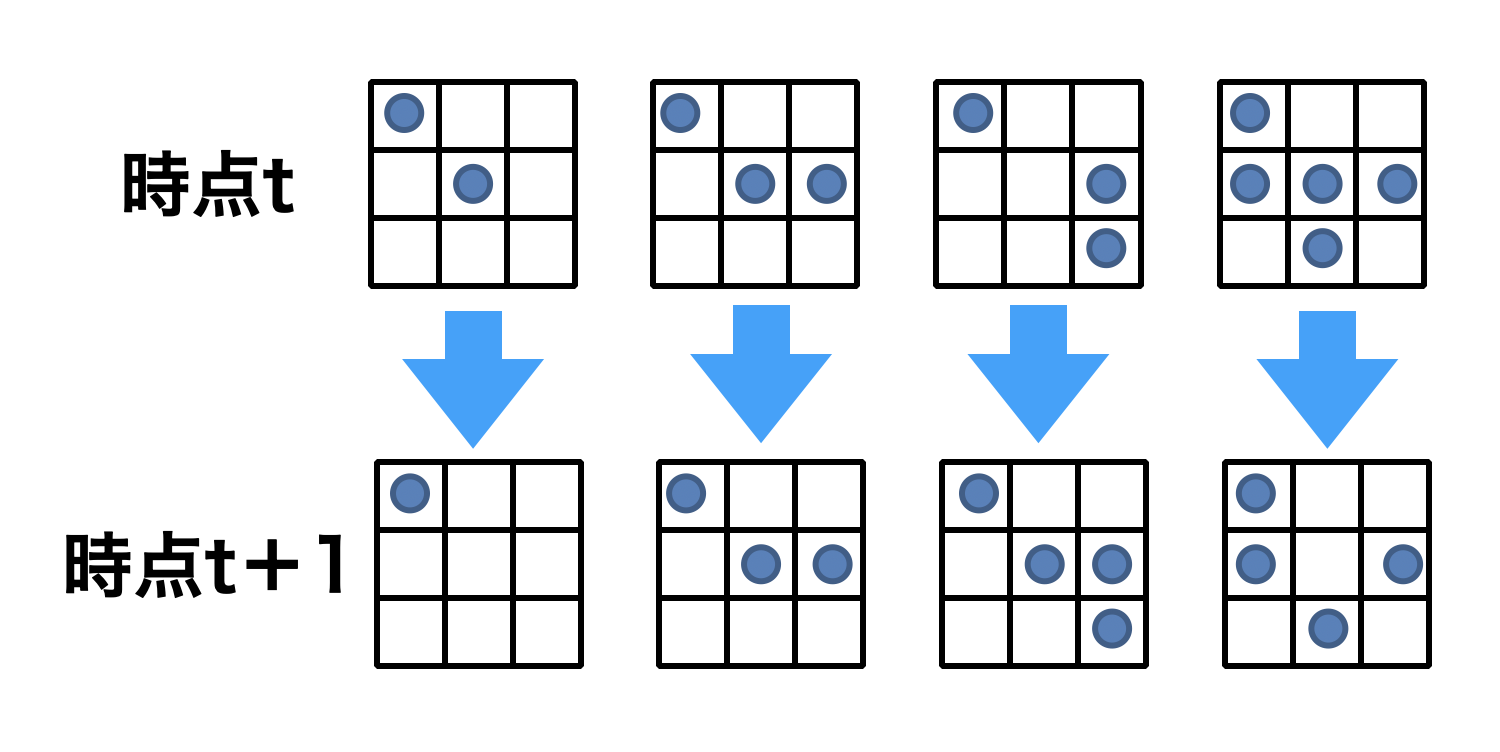
\includegraphics[keepaspectratio,width=0.7\linewidth]{../images/10_LifeGame.png}
	\caption{ライフゲームのルール}
	\label{LifeGame}
\end{figure}

ライフゲームに「ライフ」という名前が付いているのは，周りの人数が多すぎても少なすぎても生き苦しくて，黒が生きていると考えると，寂しすぎて死ぬ，多すぎて死ぬ。ちょうどいい人数だったらそのまま。3人いたら新しく生命が生まれる，という生と死のメタファーとして語られるからです。

これ，実際に見てみると，面白いパターンが現れます。例えば，グライダー\index[termidx]{ぐらいだー@グライダー}と呼ばれるパターンがあります。これを動かすと，位置を変えながら元の形に戻るサイクルを繰り返します(図 \ref{Glider})。まるで生き物が動いているように見えます。
\begin{figure}[ht]
	\centering
	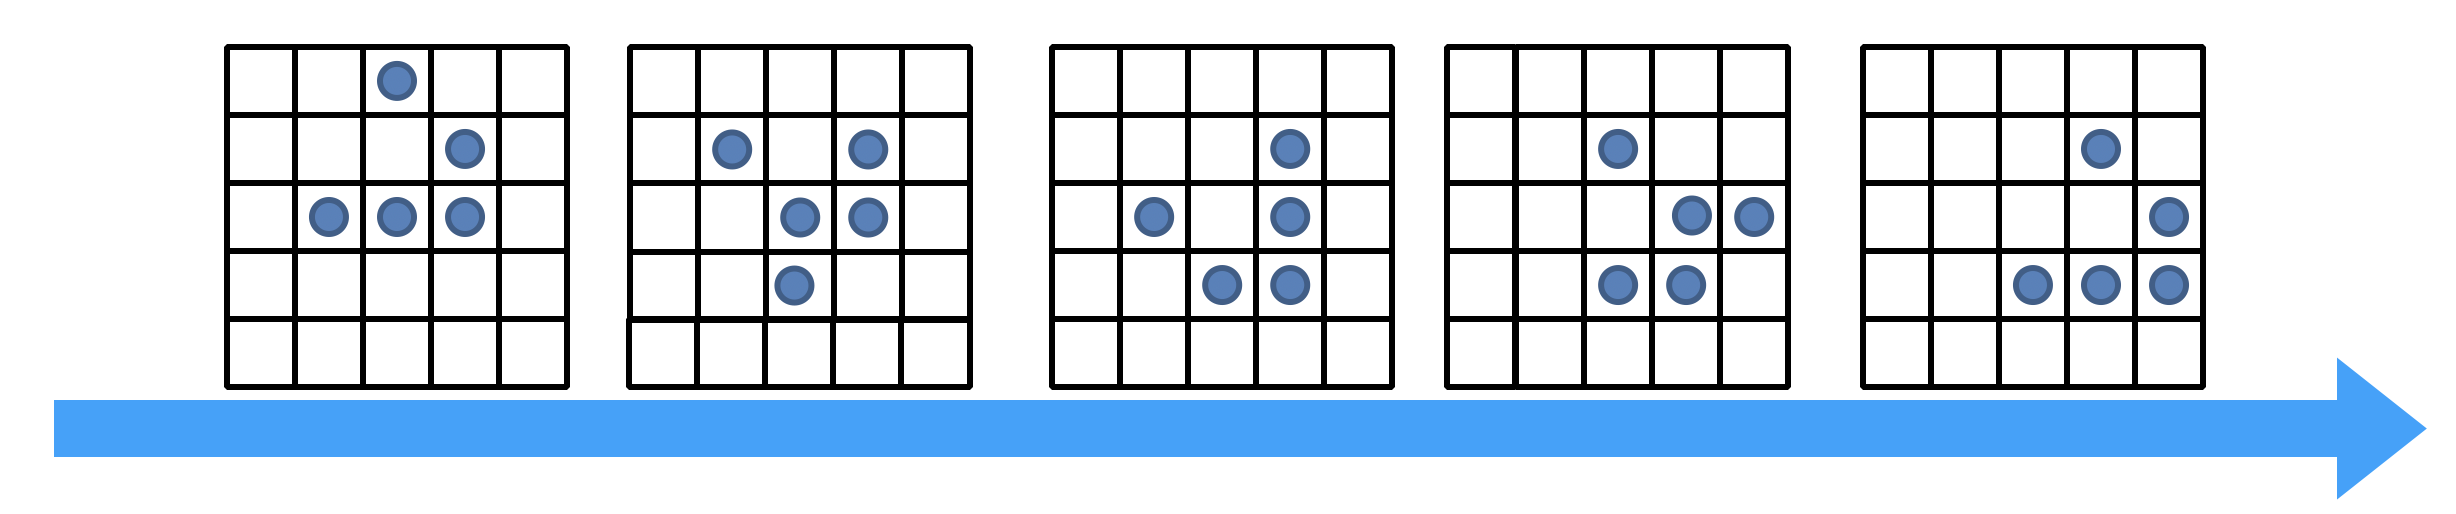
\includegraphics[keepaspectratio,width=0.7\linewidth]{../images/10_Glider.png}
	\caption{グライダー\index[termidx]{ぐらいだー@グライダー}のパターン。4ターンで少しズレた位置に同じパターンが再現される}
	\label{Glider}
\end{figure}

さらに面白いパターンとして，グライダーガン\index[termidx]{ぐらいだーがん@グライダーガン}というものがあります。これは，グライダー\index[termidx]{ぐらいだー@グライダー}を次々に生成するパターンです。他にも，宇宙船というパターンがあり，これも右に動きながら一定の周期で同じ形に戻ります。女王鉢やネブラといった，周期的に同じ形に戻ってくるパターンも存在します。

このライフゲームは，セルオートマトン\index[termidx]{せるおーとまとん@セルオートマトン}のどういうルールにすれば面白いパターンが見られるのかという研究の中で，たまたま見つかった分かりやすいパターンです。例えば，ルールを少し変えると，すぐに真っ白になったり真っ黒になったりしてしまいますが，このルールの時だけ絶妙に面白いパターンが生まれます。

今でこそコンピュータの能力が上がっていますから計算が速いですが，93年頃は，もっとゆっくりした動きでした。プルプルと震えるパターン，固定化してしまうパターン，グライダー\index[termidx]{ぐらいだー@グライダー}が飛ぶようなパターンなど，様々な挙動が見られます。

これらの動きはまるで生き物のようで，自分と同じ形のものを作ったり，それを生産し続けたりします。コンピュータサイエンスの中で，「生きているとは何か」「生きているかのような複雑なパターンはどういうルールで生まれるか」「どういうルールであれば複雑で，どういうルールであれば複雑でないか」というようなことを考える，そういうサイエンスが出てきているわけです。

個人的には，実際のところコンウェイ\index[nameidx]{こんうぇい@コンウェイ}は優秀なコンピュータを使って遊んでいただけなんじゃないかと思ったりもしますが，複雑な世界を電脳空間に生んだのがすごいところですね。これは世界を非常に単純化して表現しているんですが，自分が周りのセルの影響だけを受けて変化しているという意味では，例えば社会心理学のモデル，個人の意見は近隣の周りの人の意見を聞いて変わるんですよ，というメタファーにも使えます。あるいは，分子生物学，化学のジャンルなどでも，このセルオートマトン\index[termidx]{せるおーとまとん@セルオートマトン}は使われています。そこでは1個の分子が周りの分子とどういう関係にあった時に，どういう反応をするか，という形で表現します。つまり，ルールは世界全体で共通なんですが，1個1個のエージェントといいますか，1つ1つの単位が，自分の周囲と相互作用してパターンが変わっていく時に，全体像がどう変わるかをシミュレーションしてみせる。そこが，このセルオートマトン\index[termidx]{せるおーとまとん@セルオートマトン}というサイエンスのアプローチの面白いところなんです。

このライフゲームは，本当にただの白黒で遊んでいるだけなんじゃないかと思われるかもしれませんが，割とこの複雑な動きを見せます。ウィリアム・パウンドストーンという人が『ライフゲームの宇宙』という本\parencite{LifegaeNoUchu}を書いているので，それを読んでみてください。このライフゲームだけで本1冊書いています。

この本は面白いですよ。このグライダーガン\index[termidx]{ぐらいだーがん@グライダーガン}は同じパターンを生成していますが，このグライダー\index[termidx]{ぐらいだー@グライダー}を消すための操作もできたりします。グライダー\index[termidx]{ぐらいだー@グライダー}とグライダー\index[termidx]{ぐらいだー@グライダー}をぶつけて消すということもできます。これをビットの単位，1と0という数字を作っているものと見なして，グライダー\index[termidx]{ぐらいだー@グライダー}が消えたら1が0になっているというように見なします。このグライダー\index[termidx]{ぐらいだー@グライダー}があるかないかのパターンの列で計算をさせることができるんです。コンピュータはどんなものも0と1のビット演算しかしていないんですが，この0と1のビットの演算をグライダー\index[termidx]{ぐらいだー@グライダー}があるかないかに置き換えて，うまく設定してやると，ライフゲームでも万能計算機ができますよ，ということが書いてあるんです。興味がある人は読んでみてください。

とにかく，こういった仕組みの中で複雑そうなパターンを生むことができる，どういうのが複雑なパターンなのかということを，このライフゲームのデモは見せてくれるわけです。

\paragraph{一次元CA}

ここにウォルフラム\index[nameidx]{うぉるふらむ@ウォルフラム}\footnote{Stephen Wolfram (1959年8月29日生まれ，存命) は，イギリス出身の物理学者・計算科学者で，セルオートマトン\index[termidx]{せるおーとまとん@セルオートマトン}の研究や「A New Kind of Science」の著者として知られる。彼の研究は，単純なルールが複雑な挙動を生む自然界の法則の解明に貢献し，MathematicaやWolfram Alphaの開発者としても著名。(Wikipediaより)}という別の頭のいい人が出てきます。皆さん，Mathematicaという数学のソフト\footnote{Mathematicaは，Stephen Wolframによって1988年に開発された数学的計算ソフトウェアで，シンボリック計算，数値計算，データ可視化，アルゴリズム開発などを統合的に行えるツール。科学，工学，金融など幅広い分野で使用され，プログラミング言語Wolfram Languageを基盤としている。(Wikipediaより)}はご存知でしょうか？Mathematicaはウォルフラム\index[nameidx]{うぉるふらむ@ウォルフラム}リサーチ社が出しているんですが，それを考えたウォルフラム\index[nameidx]{うぉるふらむ@ウォルフラム}さんです。その人がセルオートマトン\index[termidx]{せるおーとまとん@セルオートマトン}を使った研究をしています。

どんな研究かというと，さっきのセルオートマトン\index[termidx]{せるおーとまとん@セルオートマトン}，セルの自動機械は，自分と周りを見るという意味で2次元空間に配列されていましたが，これを2次元ではなくて，1次元の横一直線の棒でやりましょうと考えた人なんです\footnote{同じくWolframの開発した計算知識エンジンWolfram AlphaというWebサービスがありますが(\url{https://www.wolframalpha.com/})，ここで入力バーに「rule 60」とし，セルオートマトン\index[termidx]{せるおーとまとん@セルオートマトン}のルールだと教えてやると，セルオートマトン\index[termidx]{せるおーとまとん@セルオートマトン}のデモンストレーションが始まります！}。

横一直線の棒で考えて何が楽しいかというと，横一直線にすると，自分の近傍としては左と右しかありません。だからこの3つの組みでもってルールを考えたらいいわけです。自分の左と右がどうだったら次自分がどうなるかという考え方をすればいいから，1次元のセルオートマトン\index[termidx]{せるおーとまとん@セルオートマトン}で考えないといけないルールは，000，100，010，110，001，101，011，111の時に，それぞれ次どうなるかということを書けばいいんです。これの次に白になるか黒になるかだけですから，2の8乗，256パターンあるはずです。せいぜい数えられるぐらいだから，全部試してみたらいいじゃないかというわけですね。

\begin{figure}[ht]
	\centering
	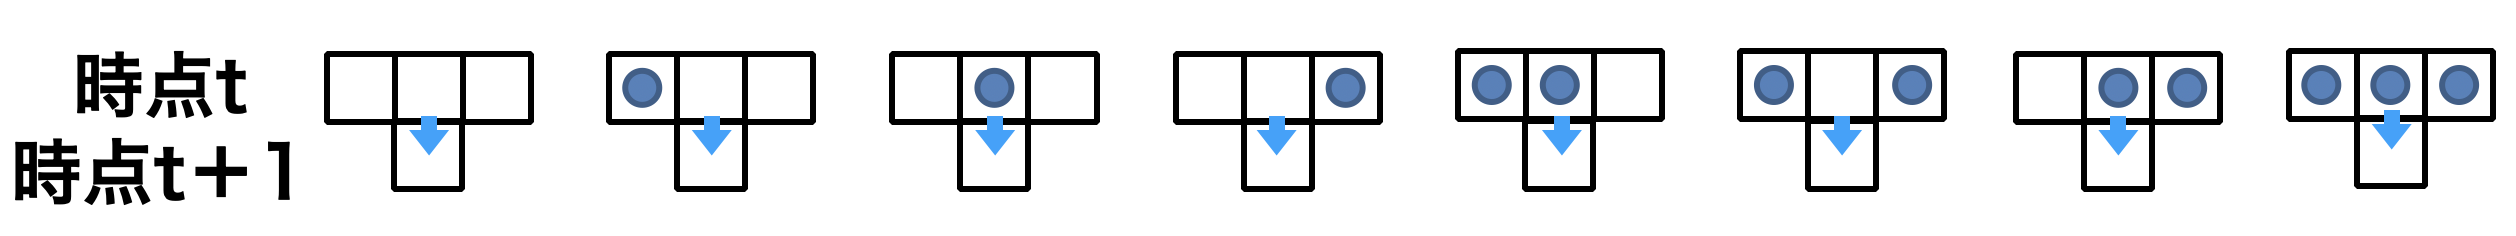
\includegraphics[keepaspectratio,width=0.7\linewidth]{../images/10_1dimCA.png}
	\caption{1次元CA。$t$時点の左右のセルの状態で$t+1$時点の自分の状態が決まる。縦軸に時間を並べて，パターンを描画する。}
	\label{1dimCA}
\end{figure}

これを全部試してみて，例えば横一線に黒黒白黒白白白，こういうパターンで，1番目のルールだったらどうなるか，2番目のルールだったらどうなるか，というようなことをやると，様々なパターンが出てきます。
ウォルフラム\index[nameidx]{うぉるふらむ@ウォルフラム}は全体を4つのパターンに分類しました：
\begin{itemize}
    \item 固定化に向かうパターン - 4世代ぐらいで次のセルを何も生まなくなる。代表的なルール番号は0, 32, 160
    \item 周期的なパターン - 同じようなパターンが繰り返される。代表的なルール番号は4, 108, 218
    \item カオス的なパターン - 一見ルールがわからない混沌とした状態。代表的なルール番号は30, 45, 90, 150
    \item カオスの縁\index[termidx]{かおすのふち@カオスの縁}パターン - カオスのようでもあり，パターンが見られるようでもある，複雑な様相を呈する状態。代表的なルール番号は110
\end{itemize}

ウォルフラム\index[nameidx]{うぉるふらむ@ウォルフラム}は1次元セルオートマトン\index[termidx]{せるおーとまとん@セルオートマトン}を全パターン計算してみて，結局のところこの4つのグループに分類したんです。定常解，周期解，カオス，そしてカオスの縁\index[termidx]{かおすのふち@カオスの縁}``the edge of chaos''というパターンがあるんじゃないかと提示しました。

\begin{figure}[ht]
	\centering
	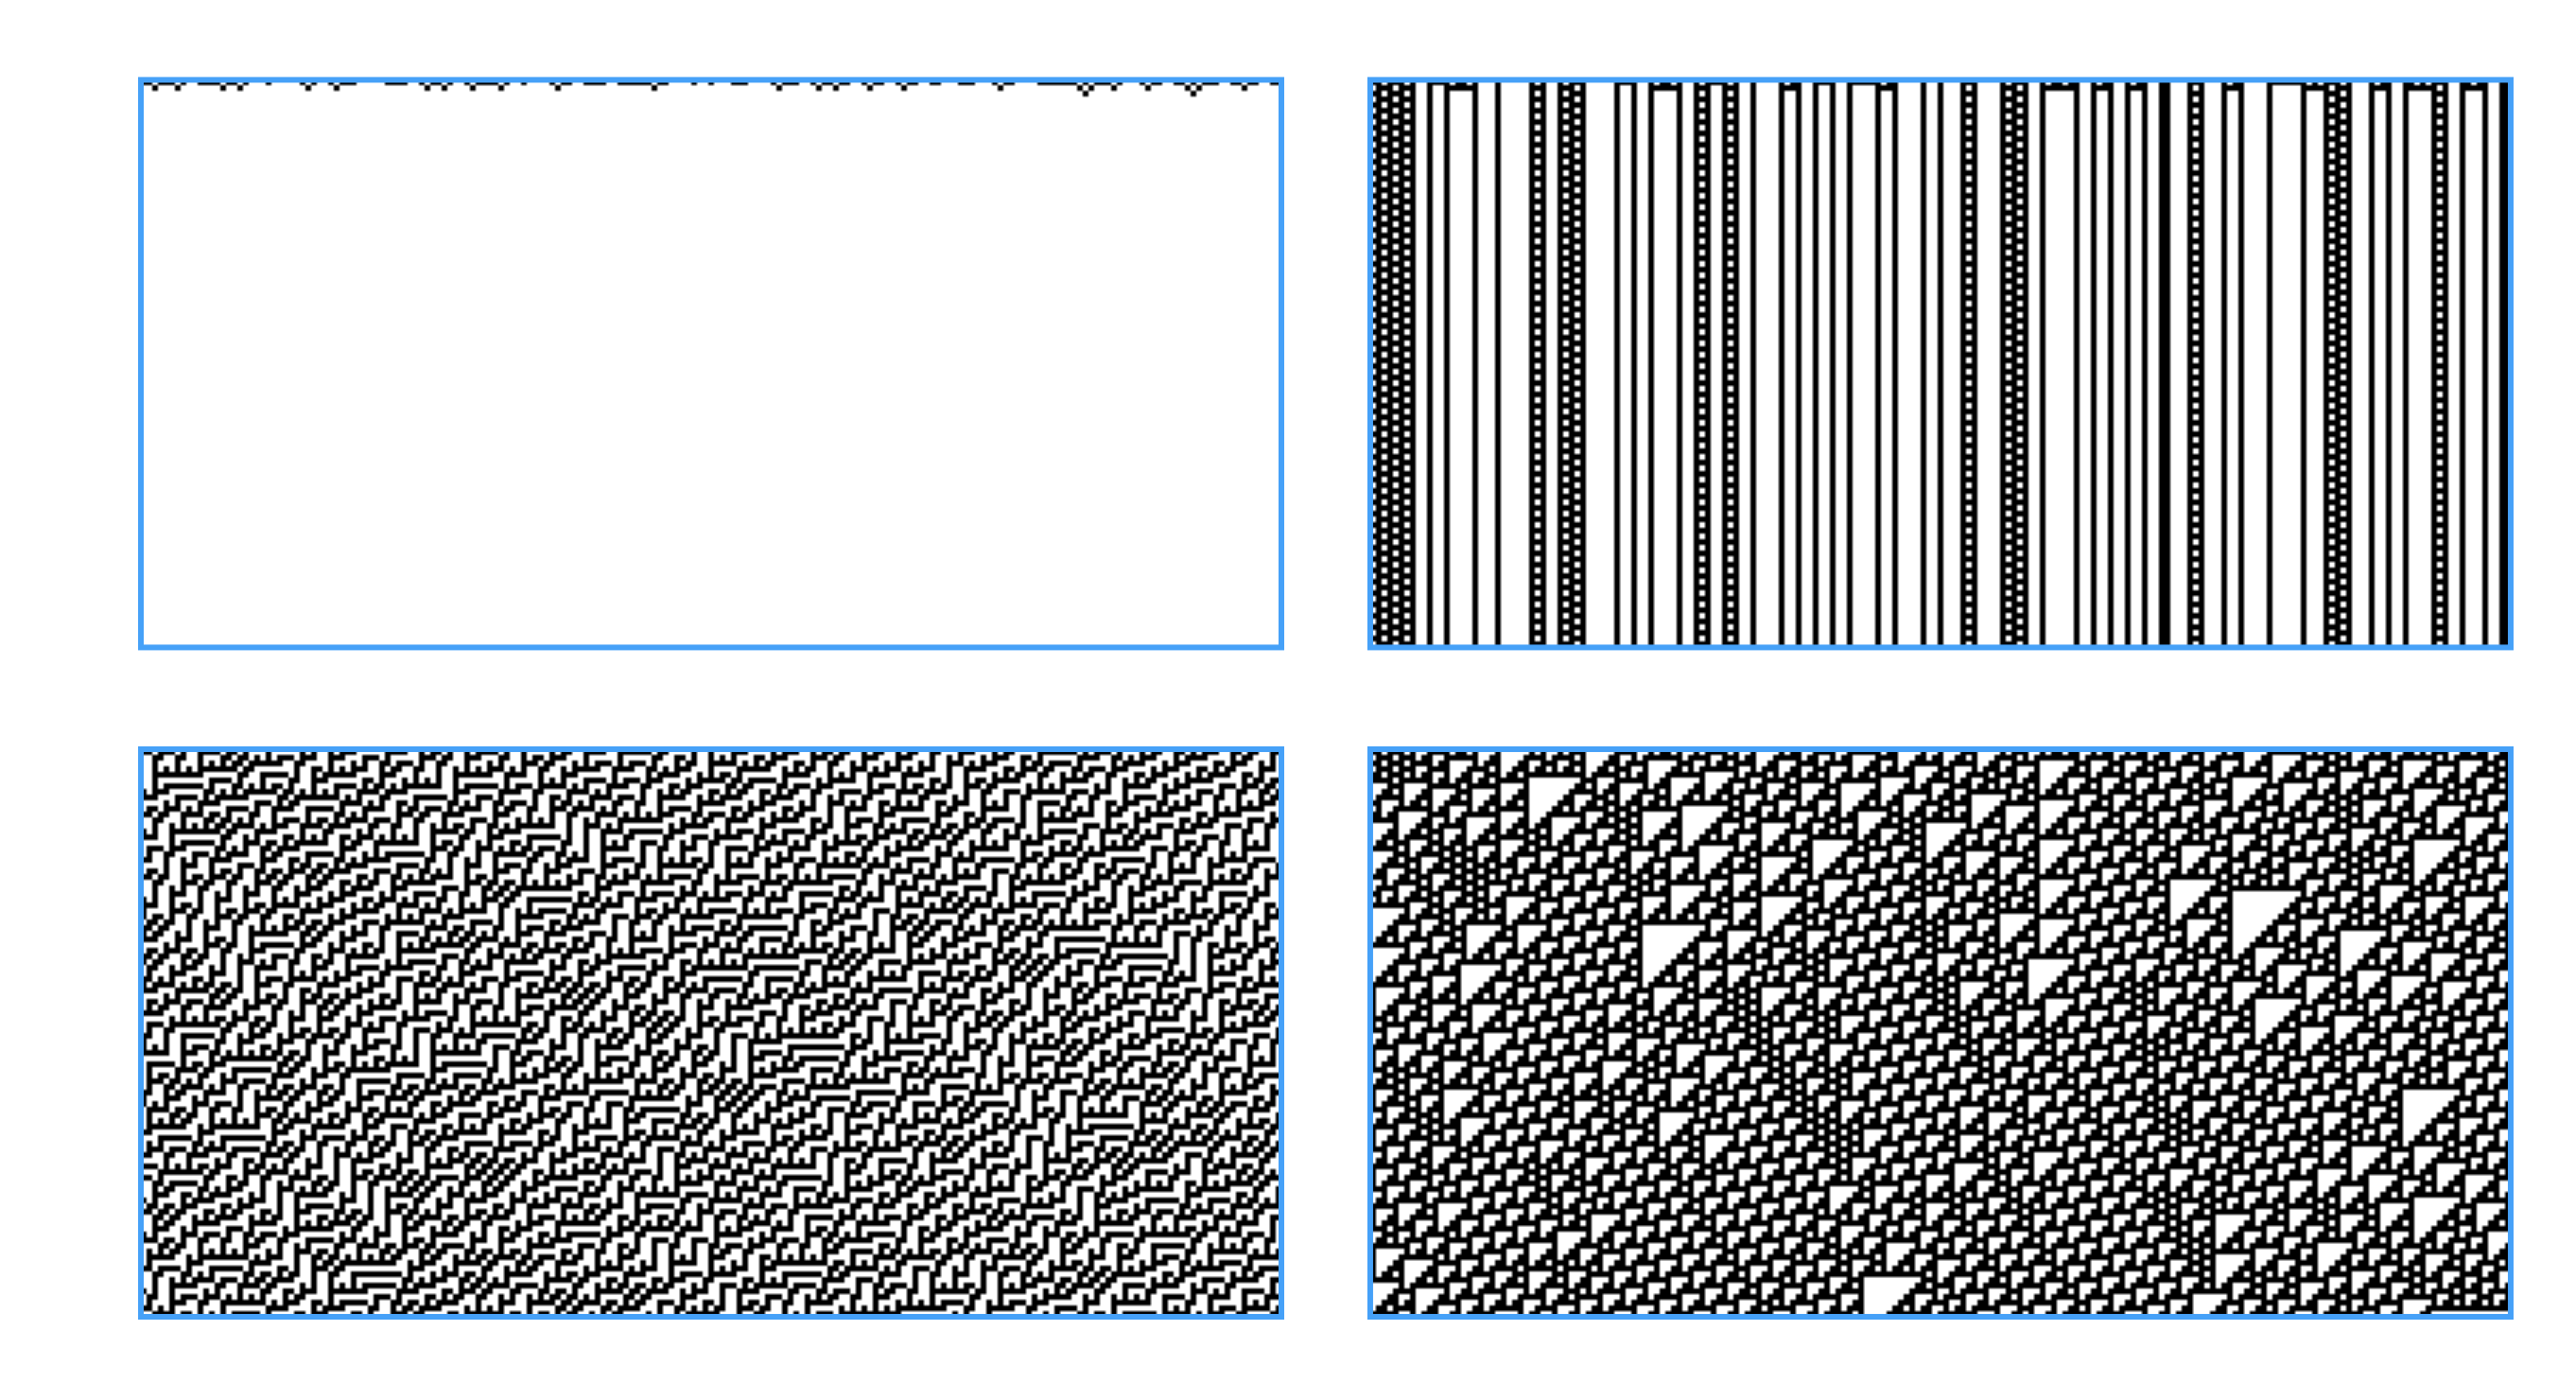
\includegraphics[keepaspectratio,width=0.7\linewidth]{../images/10_CA4pattern.png}
	\caption{4つのパターン。左上は定常解(ルール32)，右上は周期解(ルール108)，左下はカオス(ルール30)，右下はカオスの縁\index[termidx]{かおすのふち@カオスの縁}(ルール110)。Walphram Alphaで描画した。}
	\label{theEdgeOfChaos}
\end{figure}

さっきのライフゲーム(2次元セルオートマトン\index[termidx]{せるおーとまとん@セルオートマトン})は，このカオスの淵に相当していて，この時だけすごく複雑な動きをするんです。このルールの時だけ，ちょうどいい感じに複雑で単純なルールのレベルなんです。もっと単純すぎると，よーいどんで真っ白とか真っ黒になるとか，あるいは同じパターンの繰り返しだけになる。あるいは複雑すぎると，もう混沌としていて何のルールも見つからない。ライフゲームが面白いのは，ちょうどいろんなことも生まれるし生まれないしというカオスの縁\index[termidx]{かおすのふち@カオスの縁}にあるんじゃないですか，ということをデモンストレーションしているわけです。

こういうふうにコンピュータを使ったシミュレーション科学でやっていることを眺めてみると，一個一個のエージェントのルールはすごく単純なんですが，全体として複雑な様相に見えることがある。だから複雑。で，この複雑なものを全体としてこうなってるんですよと言うんじゃなくて，一個一個は単純なんだけど，それのルールの複雑さを反映して何かパターンが見えてくる。そういうようなことを扱うのが複雑系\index[termidx]{ふくざつけい@複雑系}科学だというわけです。

\paragraph{アダムループ\index[termidx]{あだむるーぷ@アダムループ}}
最後にアダムループ\index[termidx]{あだむるーぷ@アダムループ}(これはラングトン\index[nameidx]{らんぐとん@ラングトン}\footnote{Christopher G. Langton (1948年生まれ，存命) は，アメリカのコンピュータ科学者で，人工生命(Artificial Life, A-life)の研究の先駆者。生命の本質を計算モデルで探求し，ラングトン\index[nameidx]{らんぐとん@ラングトン}のループやカオスの淵(Edge of Chaos)の概念を提唱して複雑系\index[termidx]{ふくざつけい@複雑系}科学に多大な貢献を果たした。(Wikipediaより)}という人が考えたセルオートマトン\index[termidx]{せるおーとまとん@セルオートマトン}のパターン)について説明します。色が見づらいかもしれませんが，白と青と緑と赤があります。赤は鞘なのですが，「腕を伸ばせ」という命令と，ある程度時間が来たら「右に曲がれ」「左に曲がれ」とか，時間が経ったら変化しない赤い鞘になる状態があって，このパターンがとあるルールで動くとこんな風になります\footnote{このとき，授業では動画資料を投影していました。こちらのサイト\url{https://openprocessing.org/sketch/433895/}などでみることができます。}。

\begin{figure}[ht]
	\centering
	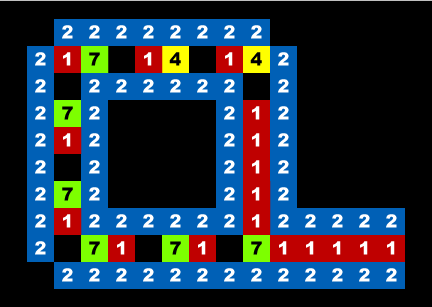
\includegraphics[keepaspectratio,width=0.7\linewidth]{../images/10_LangtonLoop.png}
	\caption{ラングトン\index[nameidx]{らんぐとん@ラングトン}のループ。アダムループ\index[termidx]{あだむるーぷ@アダムループ}ともいう。この図はWikipediaより。}
	\label{AdamLoop}
\end{figure}


時計回りの循環をするように種が配置されると，パターンがそのルールに沿って次のパターンを生み，自分と同じような形状を作ります。これは自分の複製を作っています。セルオートマトン\index[termidx]{せるおーとまとん@セルオートマトン}のグライダーガン\index[termidx]{ぐらいだーがん@グライダーガン}でグライダー\index[termidx]{ぐらいだー@グライダー}をどんどん動かすように，自分の複製を作るパターンを複製します。

これをアダムループ\index[termidx]{あだむるーぷ@アダムループ}と呼びます。これも単純なルール，単純な設定なんだけれども，あるルールに沿って単純な表現を繰り返させると，全体として非常に複雑な様相を呈する，あるいは自己を再生産する，増殖するといった特定のパターンが見えてくる例ですね。これが複雑系\index[termidx]{ふくざつけい@複雑系}の視点なんです。

さて，僕は今なんというか，言葉に悩みましたが，「複雑系\index[termidx]{ふくざつけい@複雑系}って何？」と言われたら，こんな感じのものとしか言いようがなくて，デモンストレーションを見せるというところに留まってしまいます。それは複雑系\index[termidx]{ふくざつけい@複雑系}の世界の限界ですけれども，こういったようなものが複雑系\index[termidx]{ふくざつけい@複雑系}と言われるものだということを，今ちょっとお説明したような次第です。

\subsection{複雑系の特徴}
さて，いろいろデモンストレーションを見ていただきましたが，複雑系\index[termidx]{ふくざつけい@複雑系}ってこんな感じって分かります？ちょっと総括というかまとめてみましょう。結局，複雑系\index[termidx]{ふくざつけい@複雑系}というのはどういうことが言いたいのか？

BOID\index[termidx]{ぼいど@BOID}もわかる，ベータが売れなかったのもわかる，ライフゲームで変な模様ができるのもわかる，アダムループ\index[termidx]{あだむるーぷ@アダムループ}で変な模様ができるのもわかると思うんですが，この複雑系\index[termidx]{ふくざつけい@複雑系}というようなシステム論が言いたいことは何か。

特徴づけるポイントはいくつかあるんですが，1つはシンプルなエージェントであるということですね。セルオートマトン\index[termidx]{せるおーとまとん@セルオートマトン}のセルはたった8つの周りの状態だけから，次の状態を決めるわけです。僕たちが何か人物のことを考えるときに「8人しか友達いません」なんてことはありませんよね。普通もっといろいろなところから情報を取ってくるんですが，セルオートマトン\index[termidx]{せるおーとまとん@セルオートマトン}はすごく単純化して，2次元だったら8つ，1次元だったら両横の状態から見て次の自分の状態を決める。ラングトン\index[nameidx]{らんぐとん@ラングトン}のアダムループ\index[termidx]{あだむるーぷ@アダムループ}でもそんなにパターンの数はありません。鳥のシミュレーションのBOID\index[termidx]{ぼいど@BOID}なんかに至っては，「自分は向こうに行きたい，友達とぶつかりたくない，友達と離れたくない」というたった3つのシンプルなルールです。

あともう一つのポイントとしては，局所的相互作用\index[termidx]{きょくしょてきそうごさよう@局所的相互作用}です。個々はシンプルなルールで，それが相互作用をするときに，自分の周囲しか見ていない。
この世界全体を見渡して行動するわけではありません。例えばライフゲームの世界でも，この世界全体を通じて世界のルールが決まっているんですが，ここのエージェントが気にしているのはここだけ，というように自分のごく近傍としか交渉しません。近傍を共有しているところもいっぱいあるんですけれども，全体を見て考えているんじゃなくて，せいぜい自分の周りとの関係だけから次の状態を決めますね。この一個一個は単純なルール，周りのやつがどうなったら，周りの鳥の位置がどうなったら，周りにベータ持ってる人は何人いたらとかって。個々人は単純で「あとはビデオを楽しみたい」とか「向こうに行きたい」とか。みんな単純なルールで動いているんだけれども，それが並列的に局所的な相互作用をすると全体として複雑な様相を呈する。これが複雑系\index[termidx]{ふくざつけい@複雑系}の科学の中にある基本的な発想です。

今日いくつか例を出しましたが，全体を指して複雑系\index[termidx]{ふくざつけい@複雑系}(コンプレックスシステム\index[termidx]{こんぷれっくすしすてむ@コンプレックスシステム})で表現しようとしているのは，(1)単純なエージェント，(2)局所的相互作用\index[termidx]{きょくしょてきそうごさよう@局所的相互作用}，(3)全体として複雑な様相を呈する，この3つです。こういったことから何がわかるかというと，一つはバタフライ効果みたいな，ちょっとした初期値の違い，ちょっとしたセルオートマトン\index[termidx]{せるおーとまとん@セルオートマトン}の最初の設定の違いで意外と複雑なことが起きるということです。

複雑になるかならないかみたいなパターン，セルオートマトン\index[termidx]{せるおーとまとん@セルオートマトン}の場合は周期系か定常系かカオスなのかカオスの端かという4つの状態があるんだという話をしましたが，我々の生命，生きている世界，人間社会というのはすごく複雑です。いろんなことが急に起こったり，急に何かが炎上したり，急にブームが下火になったりとか，いろんな複雑な現象が生じています。その複雑な様相を呈するギリギリのちょうどいいルール加減があるよね，というそのパターンを示す--なんて言ったらいいか，言葉が難しいな。ラングトン\index[nameidx]{らんぐとん@ラングトン}はこれを指標化して「ラムダ指標\index[termidx]{らむだしひょう@ラムダ指標}」というのを作っているんですけどね。だいたいルールの複雑さがこの程度の指標であれば一番複雑なゲームができるね，というふうなことを発見しているわけです。

\subsection{複雑系理論の特徴}
2000年の頃かな，ちょっと前なんですけどね，97，98年ぐらいがピークだったかなと思うんですけど，もうあちこちで「複雑系\index[termidx]{ふくざつけい@複雑系}は面白い」「こんなこともある」「あんなこともある」「そんなこともある」「こんなパターンもある」んで，「1個1個は単純なんだけどすごく複雑に見えるようなことっていっぱいあるね」というようなことで大ブームを巻き起こしました。いかがでしょうか？説明していてデモンストレーションを見るとね，個別のデモンストレーションはまあ「変な形が出るのは面白いな」みたいなことはあるんですけど，改めてその特徴や限界を考えてみたいと思います。

複雑系\index[termidx]{ふくざつけい@複雑系}の「システム」，Complex Systemの理論的特徴は何かというと，まず何よりもパターンから入っていることです。パターンの科学になっているということですね。

今皆さんにはグライダーガン\index[termidx]{ぐらいだーがん@グライダーガン}とか，1次元セルオートマトン\index[termidx]{せるおーとまとん@セルオートマトン}の模様とか，ラングトン\index[nameidx]{らんぐとん@ラングトン}のループとか見ていただきましたが，その前の鳥の群れとかヌーの群れとかというのも群れの動きというパターンですね。第一世代，第二世代システム\index[termidx]{だいにせだいしすてむ@第二世代システム}なんかとは違って，物理的な実態とか要素のシステム論ではなくて，もう見え方，パターンの科学になっているというところが複雑系\index[termidx]{ふくざつけい@複雑系}の大きな特徴です。でもこれはある意味弱点でもあって，平たい言い方をすると全体主義なんです。全体主義というか全体還元主義\index[termidx]{ぜんたいげんげんしゅぎ@全体還元主義}なんです。

全体的に見たら複雑に見えるよねって言っているだけであって，この要素が複雑な現象を創発\index[termidx]{そうはつ@創発}しますって言うんですけど，我々に見えているのは「いや生命って色々あるね」とか「生き物って色々なパターンがあるね，不思議だね」という表に出てきた不思議そうな見え方のところで表しているだけに過ぎないとも言えるわけですね。

さて，生きているとはどういうことか。あのラングトン\index[nameidx]{らんぐとん@ラングトン}のあのループってすごく生き物っぽいよね，ライフゲームのあのパターン生きているかのように動くよね，という「生きているとは何か」ということを考えたときに，再生するとか増殖するとか，成長するといった生き物が持っている特徴を，パターンの再生，パターンの増殖，パターンの成長という形で見せている。何らかのパターンは再生したり増殖したり成長したり(成長というのは同じ形のまま大きくなるみたいなことですけど)，そういうふうなことがあると私たちは生きているかのように見えるというわけですね。

システム論のそもそもの目的が生命とは何かを探求するための科学ですから，その話がコンピュータの空間の中でパターンの再生，増殖，成長という観点に移ったわけです。これがまず大きい。

第三世代システム\index[termidx]{だいさんせだいしすてむ@第三世代システム}，オートポイエーシス\index[termidx]{おーとぽいえーしす@オートポイエーシス}システムというのは実体によらないサイエンスになったんだという話をしましたね。物理的な実体なのではなくて，プロセスという位相空間\index[termidx]{いそうくうかん@位相空間}上の実在を要素とするシステムですね。プロセスが再生産，プロセスが繰り返されると，それがシステムなのであって，プロセスが繰り返されることによってプロセスを維持するための要素が生成されるとかいうことを考えているわけです。

つまりオートポイエーシス\index[termidx]{おーとぽいえーしす@オートポイエーシス}システムは対象としている空間がもう現実の物理の空間ではなくて，要素関係の位相空間\index[termidx]{いそうくうかん@位相空間}になっている。複雑系\index[termidx]{ふくざつけい@複雑系}も同じです。電脳空間ですけど，そこに現れるパターンの科学になっているというところがポイントです。

ただオートポイエーシス\index[termidx]{おーとぽいえーしす@オートポイエーシス}と違うのは，それが生きているように見えるということからわかるように，観察者は外部にいるということですねオートポイエーシス\index[termidx]{おーとぽいえーしす@オートポイエーシス}は観察者が内部にいるんですが，複雑系\index[termidx]{ふくざつけい@複雑系}の観察者はシステムの外から見ています。この辺が弱点といえば弱点ですけれども，複雑系\index[termidx]{ふくざつけい@複雑系}が言わんとしていることはこういうことだということですね。

2つ目の理論的特徴として，エージェント自体は単純なんだけれども，全員に共通したルールがあるとかという考え方。エージェントはその環境の世界のルールを反映しているだけであって，エージェント自体が複雑な動きをしようと思っているわけではないということです。エージェントは単純で，複雑に見えるのは環境の複雑さを反映している。環境の反映で複雑に見えるということですね。

環境って書いたのは，ライフゲイムでいうところの，更新ルールのほうです。どちらかというと，周りがいくつになったときに白で，いくつになったときに黒になるというようなルール。エージェント自体は単純でそのルールだとか環境の状態を機械的に対応しているだけですね。複雑系\index[termidx]{ふくざつけい@複雑系}は，複雑適応系と呼ばれることもあるんですけど，それはこの環境を反映している，ということを指しているようです。環境に適応するとこんな複雑なことが振る舞いに見えますよね，ということです。

だからエージェント自体はそこまで複雑なことを考えてない。例えば社会運動だとか歴史のダイナミックな動き，そう例えば，戦国時代というのは勇猛果敢でというのすごくいきいきとした表現があったりしますけど，あれって別に時代がそうだったからというのを反映しているだけで，一人一人がわざわざ複雑な何か動きをしようとしていてそうなったわけじゃないよね。

例えば織田信長の出世のストーリーとかっていうのは，本当にいろいろあって面白いですよね。家康だって昔は人質だったんだけれども，なんとか今川をやっつけて，だんだん上がっていったけど，秀吉に天下を取られて，頭を下て我慢していたかと思うと最終的には将軍になった。すごく浮き沈みのある，大変面白い物語ではあると思うけれども，エージェントとしての徳川家康は，最初からそんな複雑なルートを動こうと思ってたわけじゃないでしょう。あの時代，あの環境，あの社会に必死に自分の周りに適応しようと思ったら，あんなドラマチックな人生になったということじゃないかな，と思います。

ともかくそういう観点ですね。つまりエージェント自体が複雑なものではないということ。複雑な環境，あるいは周りの環境に適応すると複雑そうに見えた振る舞いをしているということです。最終的にその振る舞いの結果として何かのパターンが生成されているというわけですね。

そのパターンの安定というのが実はシステムの目的なんじゃないかと。複雑系\index[termidx]{ふくざつけい@複雑系}の目的，系の目的はパターンの安定です。第一世代システム\index[termidx]{だいいちせだいしすてむ@第一世代システム}というのはインプットとアウトプットを繰り返しながら，生き物としての安定。第二世代システム\index[termidx]{だいにせだいしすてむ@第二世代システム}はミクロなレベルでは不安定かもしれんけどマクロなレベルでは安定しているという話。オートポイエーシス\index[termidx]{おーとぽいえーしす@オートポイエーシス}はもう系が閉じればOK。

この観点から行くと，複雑系\index[termidx]{ふくざつけい@複雑系}は，パターンができることが目的，と言えるかもしれませんね。一人一人はパターンに関与しているんだけれども，パターンが安定するように動いていると考えたら，システムの目的はパターンの安定です。一人一人のエージェントから複雑なものが創発\index[termidx]{そうはつ@創発}してきたって言ったときに，その創発\index[termidx]{そうはつ@創発}したシステムがいかにして安定するのかっていうのが複雑系\index[termidx]{ふくざつけい@複雑系}の目指すところだったんじゃないかなと思います。

\subsection{複雑系理論の限界}
さて，最後にちょっとだけ付言をしていくというか，複雑系\index[termidx]{ふくざつけい@複雑系}の限界について話をしておきますと，皆さん今日の話面白かったですか？

複雑系\index[termidx]{ふくざつけい@複雑系}の考え方っていうのはいろんな論者がいます。でも，中心的な論者がいません。別にそのこと自体が問題なわけではないんですが，例えばオートポイエーシス\index[termidx]{おーとぽいえーしす@オートポイエーシス}はマトゥラーナとヴァレラ\index[nameidx]{ゔぁれら@ヴァレラ}という，中心的論者がいるんですね。でも，複雑系\index[termidx]{ふくざつけい@複雑系}っていうのは誰が唱えたっていうわけじゃなくて，コンピュータ科学の発展だとかもあって，みんながこういうのって面白いパターンじゃないっていいあってるやつの寄せ集めです。

だから誰が複雑系\index[termidx]{ふくざつけい@複雑系}を唱えた人ですかっていうと，そういう人は別にいません。いないことがダメと言ってるのではないですよ。ただ，そういう人がいないせいもあって，全体として複雑系\index[termidx]{ふくざつけい@複雑系}というのはこうですという，代表する論者がいないわけですね。これがひいては，理論の全体像がないことにもなってる。理論の全体像がなくて，これも複雑系\index[termidx]{ふくざつけい@複雑系}，あれも複雑系\index[termidx]{ふくざつけい@複雑系}，こんなパターンもあんなパターンも面白い。そんなふうに，20年ぐらい前にすごい盛り上がりだっただけ。言い方を変えるとみんながあちこちでデモンストレーションはするんだけれども，それを統合するような理論にならなかったんですね。だから今皆さんが複雑系\index[termidx]{ふくざつけい@複雑系}という言葉を聞いたことがない，または聞いても具体的な複雑系\index[termidx]{ふくざつけい@複雑系}の定義やら何やらが出てこないんです。みんなが「複雑系\index[termidx]{ふくざつけい@複雑系}って面白いね」と終わらせてしまったんです。

まだ終わっていない，と言うひともいるかもしれません。少なくとも現在，大学のどこかに複雑系\index[termidx]{ふくざつけい@複雑系}学部とかがあるわけじゃない。サンタフェも，今どうなってるんでしょうね。もちろん研究の結果，「それは複雑系\index[termidx]{ふくざつけい@複雑系}だ」「システムは複雑だ」という人はいますよ。でも，複雑系\index[termidx]{ふくざつけい@複雑系}理論を提唱してみんなを牽引しているという話にはなってないと思います。

だから今日の話が面白かったとしたら，デモンストレーションや断片的なエピソードが面白かったわけで，それ全体としてどうなのかという全体像が描けたか，伝えられたかが心配です。まあ，それが複雑系\index[termidx]{ふくざつけい@複雑系}の世界なんです。

私などはコンピュータの発展とともに青春時代がありましたから，例えば，ちょっと前までは本当に鳥のCGが下手だったなのが，ほんの数年で非常にリアルな動きになってきている，といった変化を目の当たりにした，という面白さはあります。VHSの論争みたいな話も身近な経験，自分の生きてきた時代の話です。電子マネーの話なんかも，VHSとベータの話を知っているからこそ，「多数を取り込んだ方が勝てる」ような戦略になったんだなと思いますし，その戦略を生み出した人が出てきているわけです。ともかく私が生きていた時代というのは，そういう意味でものすごく盛り上がって，みんな当然のように複雑系\index[termidx]{ふくざつけい@複雑系}をやり，複雑系\index[termidx]{ふくざつけい@複雑系}を通り過ぎていったというような印象があります。

\section{第五世代システムへ}

次回は第五世代の話を半分くらいやって，次の話題に進めていきたいと思います。第五世代の話は，藤澤等\index[nameidx]{ふじさわひとし@藤澤等}という人が書いた『複合システムネットワーク\index[termidx]{ふくごうしすてむねっとわーく@複合システムネットワーク}』\parencite{fujisawaNetwork}を中心にお話しします。何を隠そう，藤澤先生は私の学部の時の指導教員で，今も元気にしておられます。先日もお会いして話しました。彼は面白い人で，勢力的なおじさんですが，ずっとシステム論のことを考え，それを社会心理学の中に導入しようとした人です。

社会心理学にシステム論の発想を導入するためには，複合システム\index[termidx]{ふくごうしすてむ@複合システム}があることが必要です。それは人が複数人，含まれるからですね。そもそも複合システム\index[termidx]{ふくごうしすてむ@複合システム}でないといけない。それから，複数の人間が作るパターンの科学だとすると，オートポイエーシス\index[termidx]{おーとぽいえーしす@オートポイエーシス}だとか複雑系\index[termidx]{ふくざつけい@複雑系}の話を受けて，パターンとしての人間，パターンとしての社会システム\index[termidx]{しゃかいしすてむ@社会システム}ということを考えることになります。また一つの問題は，階層関係ですね。個人と社会という2つのレベルを考えないといけないので，社会は個人からどのようにして生まれるかということを考える必要がありますです。藤澤先生は，階層関係を前面に押し出したシステム論を考えた人です。

第五世代システム\index[termidx]{だいごせだいしすてむ@第五世代システム}のタイトルが「複合システムネットワーク\index[termidx]{ふくごうしすてむねっとわーく@複合システムネットワーク}」という言葉にあるように，システムは最初から複数があって，それがネットワークを組んでいる。このあたりは第四世代的な発想ですよね。ニューラルネットワークやセルオートマトン\index[termidx]{せるおーとまとん@セルオートマトン}みたいに，どう繋がっているかの科学であり，システム論的に社会心理学を捉えようというお話です。
その見方を見ることによって，第1回の時からずっとお話ししてきました「社会心理学という学問は一体どのような学問なのか」という問いの，システム論的な答え方のヒントが得られるのではないかなと思っております。なので，次回はその辺についてお話しできればなと思っております。

あ，もう1つだけ追加しておくと，第五世代システム\index[termidx]{だいごせだいしすてむ@第五世代システム}，複合システムネットワーク\index[termidx]{ふくごうしすてむねっとわーく@複合システムネットワーク}の特徴というかキーワードは，「境界の創出」です。どこで人がまとまりになるかということのパターンが，どこでどのように生まれるかのサイエンスなんだというところですね。これについてちょっと次回はお話しして，システム論の話を閉じて次に進んでいきたいと思っております。

はい，それでは今日の話はここまでにしておきましょう。お疲れ様でした。

\printbibliography[title=引用文献]

\end{document}

